\chapter{Prototipo 1}
  \section{Análisis}
    \subsection{Objetivo}
      Crear el módulo de conexión de datos apropiado para el manejo de la información de acuerdo a un modelo de datos propuesto diseñado por el equipo de trabajo.

    \subsection{Características}
      \begin{itemize}
        \item El modelo de datos propuesto deberá satisfacer las necesidades para trabajar con diferentes artículos y la interacción con sus usuarios.
        \item El sistema deberá permitir la conexión a la fuente de datos que corresponda con el modelo propuesto.
        \item El sistema deberá ser capaz de realizar operaciones sobre los datos de la fuente para el correcto funcionamiento de los procesos lógicos del sistema.
      \end{itemize}

    \subsection{Restricciones}
      \begin{itemize}
        \item El sistema se verá limitado por el lenguaje de desarrollo Java.
        \item Para el caso de estudio, el sistema operará con el gestor de base de datos propio de Neo4j. 
      \end{itemize}

  \section{Diseño}
    \subsection{Modelo de datos}
      Para la API, el problema fundamental recae en que las recomendaciones pueden ser utilizadas para diversos casos de estudio, buscando una generalización de las características mínimas requeridas para realizar recomendaciones se plantea un modelo de datos utilizando tres principales entidades: Usuarios, Artículos a recomendar, y Categorías como características que permitan clasificar los diferentes artículos. La información que será guardada y posteriormente consultada por otros módulos del sistema seguirá un esquema propuesto por el equipo de trabajo, éste recopila la estructura de evaluaciones básicas generadas en prácticamente cualquier tipo de artículos, películas, platillos, libros, entre otros como podemos ver en el siguiente diagrama de grafos.

      \newpage
          \begin{landscape}
            \begin{figure}[h!]
            \centering
            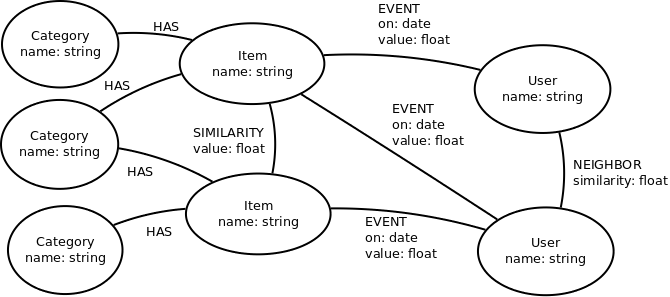
\includegraphics[width=22.5cm,height=12cm]{./images/general_data_model.png}
            \caption{Modelo general necesario para el manejo de la información}
          \end{figure}
          \end{landscape}
        \newpage

      Para la aplicación cliente correspondiente al caso de estudio de recomendación de platillos, el sistema tendrá un modelo de datos que parte del modelo general mínimo necesario para trabajar la información añadiendo información relevante sobre el caso de estudio que recae en platillos como artículos a recomendar. Considerando al final las siguientes entidades.
      \begin{itemize}
        \item Platillos
        \item Usuarios
        \item Restaurantes
        \item Categorías
      \end{itemize}

      El siguiente diagrama muestra las entidades utilizadas en el sistema de recomendación de platillos así como las relaciones existentes entre las mismas. En éste los nodos del grafo corresponden a las entidades Usuario, Platillo, Restaurante y Categoría. Donde las relaciones entre ellos se describen de la siguiente manera: 
      \begin{itemize}
        \item Un platillo puede ser de una o más categorías.
        \item Un platillo puede ser servido en uno o más restaurantes
        \item Un usuario puede agregar un platillo
        \item Un usuario puede interactúar con un platillo a través de un conteo de clics.
        \item Un usuario puede evaluar qué tanto le gustó un platillo a través de un rating cuantitativo.
      \end{itemize} 


      \begin{landscape}
        \begin{figure}[h!]
          \centering
          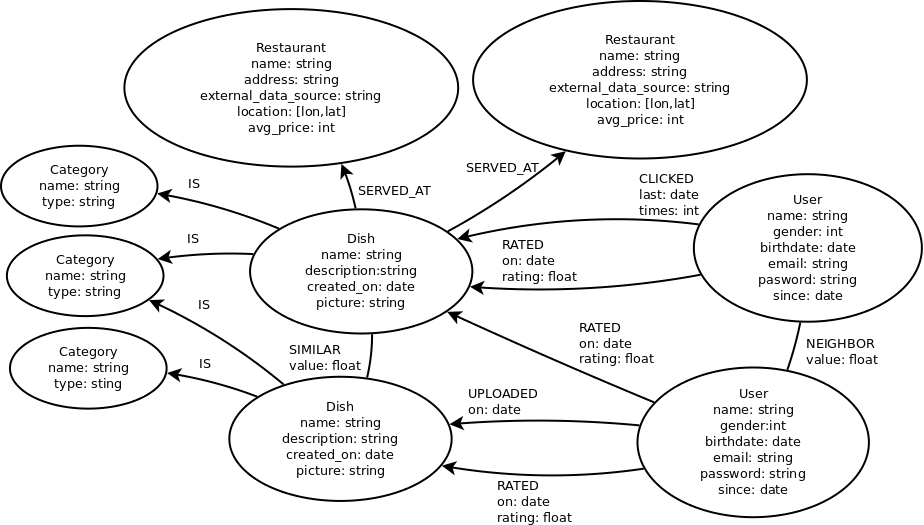
\includegraphics[width=22.5cm,height=12cm]{./images/sc_data_model.png}
          \caption{Modelo de datos propuesto para el caso de estudio}
        \end{figure}
      \end{landscape}

  \section{Resultados}
    Como resultado de la implementación del modelo de datos para el sistema podemos ver la siguiente representación gráfica del modelo utilizado en el caso de estudio. 
            \begin{figure}[h!]
            \centering
            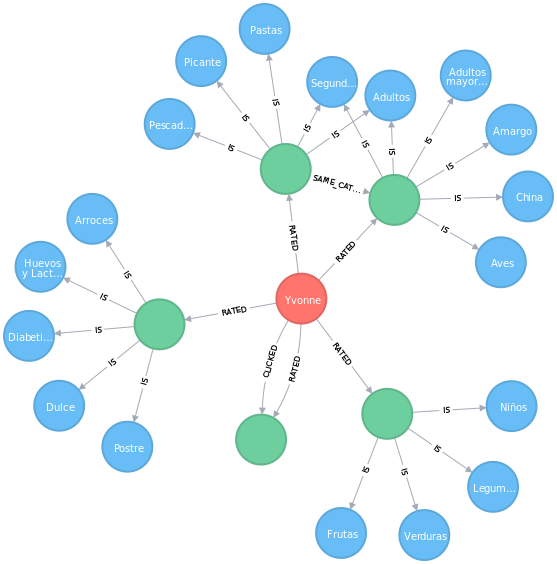
\includegraphics[width=12cm]{./images/graph}
            \caption{Modelo de datos implementado para el caso de estudio}
          \end{figure}
